\documentclass[conference]{IEEEtran}
\IEEEoverridecommandlockouts
\usepackage{cite}
\usepackage{amsmath,amssymb,amsfonts}
\usepackage{graphicx}
\usepackage{textcomp}
\usepackage{xcolor}
\usepackage{booktabs}
\usepackage{array}
\usepackage{tikz}
\usetikzlibrary{positioning,arrows.meta,shapes.geometric}

\def\BibTeX{{\rm B\kern-.05em{\sc i\kern-.025em b}\kern-.08em
    T\kern-.1667em\lower.7ex\hbox{E}\kern-.125emX}}

\begin{document}

\title{Structure-Aware Retrieval for ISO Standard Documents:\\
A Comparative Study of Chunking and Retrieval Strategies}

\author{\IEEEauthorblockN{[Student Name]}
\IEEEauthorblockA{\textit{[Department Name]} \\
\textit{[University Name]}\\
[City, Country] \\
[email@example.com]}
\and
\IEEEauthorblockN{[Guide Name]}
\IEEEauthorblockA{\textit{[Department Name]} \\
\textit{[University Name]}\\
[City, Country] \\
[email@example.com]}}

\maketitle

\begin{abstract}
Electric vehicle charging and vehicle-to-grid communication are governed by the ISO 15118 standard family, a set of long, densely cross-referenced engineering documents containing exact message names, field identifiers, normative tables and clause dependencies. Large language models (LLMs) answer technical questions fluently but frequently produce unsupported statements because their parametric knowledge does not reliably cover exact identifiers and clause-level detail. Retrieval-Augmented Generation (RAG) grounds generation in retrieved passages, yet conventional RAG over engineering standards still suffers retrieval failure (fragmented passages, tables split mid-row, lost clause relationships) and generation failure (answers unsupported by the retrieved evidence). This paper develops a fully local RAG question-answering system over three ISO 15118 part documents and evaluates it as a controlled comparison of three chunking $\times$ retrieval ``pairings'': Pairing~1 (recursive chunking with parent-child retrieval) as the baseline; Pairing~2 (section-aware chunking with hybrid dense/BM25 retrieval fused by Reciprocal Rank Fusion); and Pairing~3 (table-first chunking with a NetworkX cross-reference graph, metadata-filtered retrieval and cross-encoder reranking). Documents are parsed with Docling, which supplies the heading, annex and table labels that drive structure-preserving chunking. Evaluation uses a 32-query gold set with deterministic retrieval metrics, an LLM-as-judge and a deterministic citation-accuracy metric. Measured first-run results show Pairing~3 achieves the best retrieval quality (Recall@5 = 1.0, MRR = 0.9307) while Pairing~2 achieves the best generation quality and latency (citation accuracy 0.96, end-to-end 2660~ms). The principal contribution is a reproducible, evidence-disciplined pipeline and evaluation harness demonstrating how structure-aware chunking, hybrid retrieval and cross-reference reasoning improve grounded question answering over engineering standards.
\end{abstract}

\begin{IEEEkeywords}
Retrieval-augmented generation, information retrieval, document parsing, hybrid retrieval, reciprocal rank fusion, reranking, question answering, ISO 15118.
\end{IEEEkeywords}

\section{Introduction}
Modern electric vehicles do not charge in isolation. In a vehicle-to-grid (V2G) deployment, the vehicle and the charging station negotiate charging parameters and coordinate energy flow through a standardized communication interface. The ISO 15118 standard family~\cite{iso15118} specifies this interface: Part~1 defines general information and use-case terminology, Part~2 defines the protocol and message layers, and Part~3 defines the physical and data-link layer requirements.

Documents of this kind have a characteristic structure. They are organized as numbered clauses nested in a hierarchy, they contain normative tables whose rows carry binding requirements, they use exact technical identifiers (message names, field names, acronyms, signal names) that must be reproduced without alteration, and they reference other clauses and annexes by number. An engineer consulting the standard asks precise questions: which message carries a given field, what a specific acronym expands to, which clause governs a given procedure, or what a table row requires. Answering such questions correctly requires locating the governing clause, not paraphrasing it.

LLMs have strong fluency and broad parametric knowledge, but their knowledge is fixed at training time and does not reliably cover the exact identifiers, clause numbers and table-level detail of a specific, versioned engineering standard. RAG~\cite{lewis2020} addresses this by retrieving relevant passages and conditioning generation on them, so that answers can be checked against, and cited to, the retrieved evidence. The quality of a RAG system is bounded by two stages that can fail independently. \emph{Retrieval failure} occurs when the retriever returns passages that are irrelevant, incomplete or fragmented---for example, when a normative table is split mid-row, or when the retriever matches surface similarity but misses the governing clause. \emph{Generation failure} occurs when the retrieved evidence is adequate but the generator produces statements the evidence does not support, or omits the citations that make the answer verifiable. These failure modes require different remedies, and a central design principle of this work is that the two stages must be measured separately.

Applying RAG to engineering standards is materially harder than applying it to general prose, for five reasons: (i) long documents with deep clause hierarchies defeat fixed-size splitters; (ii) exact technical identifiers are under-ranked by dense semantic retrieval but well served by lexical retrieval; (iii) normative tables are fragmented by generic splitters; (iv) requirements depend on other clauses, so a single matching clause is an incomplete unit of evidence; and (v) even with adequate evidence, a small local LLM may produce unsupported statements.

The problem addressed is therefore: given the three ISO 15118 part documents as PDFs, design, implement and evaluate a fully local RAG question-answering system that (a) parses the documents into structure-preserving units retaining clause identity and table atomicity, (b) retrieves the passages that govern a question, including passages reached through clause cross-references, (c) generates answers grounded in the retrieved evidence and citing their source clauses, and (d) measures retrieval quality and generation quality separately with a reproducible harness. The central research question is: \emph{which combination of chunking strategy and retrieval mechanism yields the best clause-accurate retrieval and the best grounded generation over the ISO 15118 corpus?}

The contributions are: (1) structure-aware chunking derived from parser labels rather than fixed token windows, with table atomicity; (2) a three-pairing empirical comparison over a shared ingestion substrate; (3) a deterministic cross-reference graph with retrieval expansion; (4) a deterministic citation-accuracy metric; and (5) a reproducible evaluation harness that records uncomputable metrics as flagged rather than omitted.

\section{Related Work}
\textbf{RAG foundations.} Lewis et al.~\cite{lewis2020} augment a parametric encoder--decoder with a differentiable non-parametric retriever, establishing the retrieve-then-generate pattern and showing that retrieval quality drives answer quality. Their setup assumes a web-scale corpus and gives no mechanism for citing a source; this work keeps the pattern but replaces the learned retriever with an explicit, inspectable hybrid pipeline and adds a citation requirement.

\textbf{Dense and sparse retrieval.} Karpukhin et al.~\cite{karpukhin2020} encode questions and passages independently into a dense vector space, showing that dense retrieval beats lexical baselines on open-domain QA. Robertson and Zaragoza~\cite{robertson2009} give a probabilistic account of lexical ranking that yields BM25 with term-frequency saturation and length normalisation. Reimers and Gurevych~\cite{reimers2019} make pre-computed semantic search practical with Sentence-BERT. Gao et al.~\cite{gao2023} instruction-tune a bi-encoder for zero-shot retrieval in unlabelled domains. Dense retrieval matches meaning but under-ranks exact identifiers; BM25 matches surface form but fails on paraphrase; neither alone suffices, which motivates hybrid retrieval.

\textbf{Rank fusion.} Cormack et al.~\cite{cormack2009} combine ranked lists by summing a reciprocal function of each document's rank, requiring no score normalisation or training. This work uses reciprocal rank fusion as the hybrid combination rule.

\textbf{Parsing and chunking.} Docling~\cite{docling2024} produces layout-aware output from PDFs, recognising tables as structured objects. It is a system description, not a chunking study, and does not address the externally defined clause hierarchy of a standard; this work derives a clause outline from the parser's structured labels.

\textbf{Reranking.} ColBERT~\cite{khattab2020} uses token-level late interaction to approach cross-encoder quality at lower cost, but its index is large. The BAAI \texttt{bge-reranker-v2-m3} cross-encoder~\cite{bge2024} scores query--passage pairs jointly and supports long inputs. This work uses the cheaper cross-encoder as a second pass over the top candidates.

\textbf{Graph retrieval.} Edge et al.~\cite{edge2024} build an entity--relation graph by prompting an LLM at ingestion time for query-focused summarisation. This work instead builds a deterministic, citation-derived graph whose edges are the standard's own ``see 4.2'' and ``Annex A'' references.

\textbf{Evaluation.} RAGAS~\cite{es2024} defines reference-free LLM-judged faithfulness and relevance metrics. These are non-deterministic and judge-dependent; this work implements a custom, constrained judge and adds a deterministic citation-accuracy metric.

\textbf{Research gap.} The literature establishes each component individually, but not how they behave when combined on a small, fixed, table-heavy standard. The evidence base is dominated by web, news and open-domain QA text, where passages are short and self-contained. Structure-aware chunking, table integrity, standards cross-references, joint ablation, reproducible local evaluation and citation-level verification are each under-addressed. This work responds by fixing one corpus, one ingestion path and one harness, and varying only the chunking and retrieval design across three pairings.

\section{System Requirements}
The system is a fully local RAG question-answering system over the three ISO 15118 part documents. It is organized as an ingestion stage (PDFs to stored chunks), a retrieval stage (question to ranked clauses) and a generation stage (clauses to a cited answer), wrapped by an evaluation harness and a Streamlit interface. The functional requirements are grouped by stage: ingestion (parse with Docling, cache the parse, strip headers/footers, recover the clause outline, attach metadata, provide three chunking strategies, keep tables atomic, extract cross-references, index with local embeddings, batch vector-store writes, rebuild on change); retrieval (hybrid dense/BM25 fusion, graph expansion, guarded reranking, metadata filtering, return \texttt{TOP\_K}=5 clauses); generation (answer only from context, require a clause citation, condense follow-ups, show retrieved passages); evaluation (deterministic retrieval metrics, LLM-as-judge, deterministic citation accuracy, flag uncomputable scores); and operation (fully offline, three-view UI, one pipeline at a time).

The non-functional requirements cover performance (interactive latency within a few seconds on CPU-class hardware, designed for an 8~GB machine), reliability (cached parses, graceful reranking degradation, index-freshness checks), privacy (all retrieval local; only the optional chat completion may use a network), usability, maintainability (adding a pairing requires one chunker, one retriever and one registry branch), testability (a fast, model-free suite), reproducibility (fixed corpus, temperature~0 judge, persisted JSON results) and portability (CUDA, Apple MPS or CPU). The system is constrained to a fixed corpus, no OCR by default, an 8~GB memory ceiling, and licensed material that must not be reproduced extensively.

\section{Proposed Methodology}
\subsection{Architecture and Workflow}
The architecture is layered so that the parsing and chunking substrate is shared by all three pairings; a measured difference between pairings is therefore attributable to chunking and retrieval rather than to parsing. Fig.~\ref{fig:arch} shows the pipeline. The workflow proceeds in eight steps: corpus preparation, structure recovery, chunking, indexing, retrieval, generation, evaluation and presentation.

\begin{figure}[t]
\centering
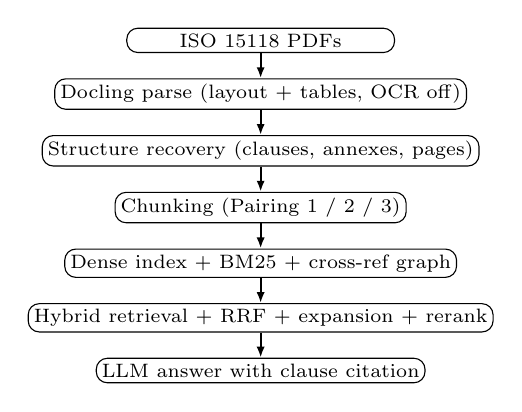
\begin{tikzpicture}[
  node distance=3.2mm,
  box/.style={draw, rounded corners, align=center, font=\scriptsize, inner sep=2pt, minimum width=3.4cm},
  arr/.style={-{Latex[length=1.4mm]}, thick}
]
\node[box] (a) {ISO 15118 PDFs};
\node[box, below=of a] (b) {Docling parse (layout + tables, OCR off)};
\node[box, below=of b] (c) {Structure recovery (clauses, annexes, pages)};
\node[box, below=of c] (d) {Chunking (Pairing 1 / 2 / 3)};
\node[box, below=of d] (e) {Dense index + BM25 + cross-ref graph};
\node[box, below=of e] (f) {Hybrid retrieval + RRF + expansion + rerank};
\node[box, below=of f] (g) {LLM answer with clause citation};
\draw[arr] (a)--(b); \draw[arr] (b)--(c); \draw[arr] (c)--(d);
\draw[arr] (d)--(e); \draw[arr] (e)--(f); \draw[arr] (f)--(g);
\end{tikzpicture}
\caption{Overall system architecture (ingestion, indexing, retrieval, generation).}
\label{fig:arch}
\end{figure}

\subsection{Ingestion and Structure Recovery}
Each PDF is parsed with Docling~\cite{docling2024} in layout-aware mode with OCR disabled, cached as JSON, and kept as a single document whose page boundaries are derived from a form-feed placeholder. A structure-recovery pass turns Docling's \texttt{section\_header} and \texttt{TableItem} labels into a clause-level outline: numeric clauses (e.g.\ 4.1.2) and annex labels (e.g.\ A, A.1) are normalised, a heading emitted as two consecutive headers is merged into one clause number and title, and furniture and front-matter headings are dropped. Recovering structure from parser labels rather than a Markdown heading regex is essential: a regex misses annexes and non-numeric headings and collapses the document into oversized sections.

\subsection{Chunking Strategies}
Three strategies consume the same structured corpus. \textbf{Pairing~1 (baseline)} uses a recursive splitter producing child chunks (256 characters, overlap 25) for matching and parent chunks (1024, overlap 100) for context; it carries no clause metadata. \textbf{Pairing~2} aligns chunks to section boundaries (512, overlap 50) so each chunk carries its section identity. \textbf{Pairing~3} produces standalone table chunks with captions, clause-level text chunks, and records cross-references. Table atomicity is a shared constraint: \texttt{pack\_units()} fills a character budget with whole units, and \texttt{split\_table\_markdown()} breaks an oversized table (above \texttt{TABLE\_MAX\_CHARS}=4000) on row boundaries while repeating the header, so a table is never fragmented mid-row.

\subsection{Metadata, Indexing and Retrieval}
Every chunk carries \texttt{document\_id}, \texttt{section\_number}, \texttt{section\_title}, \texttt{heading\_path}, page number, \texttt{content\_type} and (Pairing~3) \texttt{cross\_references}. Chunks are embedded with the local instruction-aware model \texttt{Qwen/Qwen3-Embedding-0.6B}; the wrapper applies the model's query prompt to queries only and flattens Markdown tables before encoding while leaving stored text unchanged. For Pairings~2 and~3 a BM25 index is built over the same chunk texts. Hybrid retrieval fuses the dense and sparse rankings by reciprocal rank fusion~\cite{cormack2009}: for a document $d$ and rankers $R$,
\begin{equation}
\text{RRF}(d) = \sum_{r \in R} \frac{1}{k + \text{rank}_r(d)},
\end{equation}
where $\text{rank}_r(d)$ is the 1-based rank of $d$ in ranker $r$'s list and $k$ is a damping constant. The fused list is truncated to \texttt{TOP\_K}=5; the vector and BM25 weights are 0.6 and 0.4.

Pairing~3 adds three mechanisms. A deterministic cross-reference graph is built as a NetworkX \texttt{DiGraph} whose node ids are \texttt{\{document\_id\}:\{section\}\_\{md5[:8]\}} and whose edges are the standard's own references; a bounded breadth-first expansion pulls in clauses a matched clause depends on. Metadata-filtered retrieval (SelfQuery) derives clause constraints from the question. Finally, a cross-encoder~\cite{bge2024} reranks the top \texttt{RERANK\_TOP\_N}=20 candidates and returns the top 5, guarded so that a resource failure degrades to the unranked list.

\subsection{Generation and Evaluation}
Generation is a LangChain LCEL chain: a condensation chain rewrites a follow-up into a standalone question, and the answer chain confines the answer to the supplied context, requires a document and clause citation, and instructs the model to state that it lacks sufficient information otherwise. The default chat model is a local \texttt{llama3.2:3b-instruct-q4\_K\_M} served through Ollama, with an optional OpenAI provider. Evaluation scores all pairings on the same gold set with the same judge configuration. Retrieval metrics (Recall@$k$, Precision@$k$, nDCG@$k$, MRR) are deterministic and answer-term based, with a section-based signal where clause metadata is available. Generation metrics (faithfulness, answer relevance, answer correctness) are LLM-as-judge scores at temperature~0, and citation accuracy is deterministic, computed by comparing the clause numbers cited in the answer with the sections actually retrieved. Uncomputable scores are recorded as \texttt{None} and flagged.

\section{Implementation}
The system is implemented in Python~3.12 and runs on a single 8~GB workstation; device resolution is \texttt{cuda} $>$ \texttt{mps} $>$ \texttt{cpu}. The repository is organized into packages by responsibility: \texttt{ingestion/} (loader, structure recovery, chunk helpers, three chunkers), \texttt{vectorstore/} (batched, sanitised Chroma writes), \texttt{retrieval/} (three retrievers), \texttt{graph/} (cross-reference graph), \texttt{chain/} (LCEL chains), \texttt{models/} (device, embeddings, reranker, cached chat clients), \texttt{eval/} (gold set, metrics, judge, runners, reports), \texttt{ui/} (Streamlit application and pipeline registry), \texttt{scripts/} (chunk diagnostic) and \texttt{tests/} (fast, model-free unit tests). All vector-store writes go through a single batched helper that enforces Chroma's upsert cap and strips metadata Chroma rejects. The pipeline registry constructs one pipeline at a time and releases it before building the next in compare mode, because holding all three simultaneously was out-of-memory. The test suite uses fabricated Docling items and stub embeddings, so it runs in seconds without loading models or parsing PDFs. All core components of the three pairings, the evaluation harness and the interface are implemented; NLI-based grounding, adaptive-$k$ selection, multi-run variance and incremental indexing are deferred to future work.

\section{Results and Discussion}
\subsection{Experimental Setup}
The experiment compares the three pairings on a common 32-query gold set spanning six categories: definitional (14), procedural (6), parameter lookup (5), cross-reference (2), annex lookup (2) and comparison (2). Each entry records the question, a gold answer, answer terms for deterministic relevance matching, and gold clause references. All components ran locally. Each pairing was evaluated with a single run, so the results are point measurements without variance.

\subsection{Retrieval Results}
Table~\ref{tab:retrieval} presents the retrieval metrics at $k=5$. Pairing~3 achieves the best retrieval quality on every answer-term metric: Recall@5 = 1.0000, nDCG@5 = 0.9401 and MRR = 0.9307. Pairing~1 is second on nDCG@5 and MRR, and Pairing~2 is second on Precision@5. The section-based signal, available only for Pairings~2 and~3, shows Pairing~3 at Recall@5 = 1.0000 and Pairing~2 at 0.9062. The result is consistent with the design rationale: the cross-encoder reranker promotes the governing clause above superficially similar passages, and graph expansion pulls in dependent clauses, raising recall to 1.0. Pairing~2's lower nDCG@5 and MRR relative to the baseline show that structure-aware chunking alone does not guarantee a better ranking---chunking quality and ranking quality are separable.

\begin{table}[t]
\caption{Retrieval Metrics at $k=5$}
\label{tab:retrieval}
\centering
\begin{tabular}{lccc}
\toprule
Metric & Pairing 1 & Pairing 2 & Pairing 3 \\
\midrule
Recall@5 & 0.9375 & 0.8750 & \textbf{1.0000} \\
Precision@5 & 0.5437 & 0.6062 & \textbf{0.7188} \\
nDCG@5 & 0.8920 & 0.8363 & \textbf{0.9401} \\
MRR & 0.9010 & 0.8529 & \textbf{0.9307} \\
Recall@5 (section) & N/A & 0.9062 & \textbf{1.0000} \\
\bottomrule
\end{tabular}
\end{table}

\subsection{Generation and Citation Results}
Table~\ref{tab:generation} presents the generation metrics. Pairing~2 achieves the best generation quality on all three judged dimensions: faithfulness 0.5690, answer relevance 0.6910 and answer correctness 0.7010. Pairing~3 is close on answer relevance (0.6950) but lower on faithfulness (0.4878) and answer correctness (0.5269). Pairing~1 is lowest on all three. On citation accuracy, Pairing~2 achieves 0.9600 and Pairing~3 achieves 0.9481; Pairing~1 records 0.0000, because its chunks carry no section metadata, so the clause numbers cited in its answers cannot match the retrieved sections.

The generation result is the most interesting finding. Pairing~3 wins retrieval but does not win generation: its faithfulness and answer correctness are lower than Pairing~2's, even though its retrieved evidence is at least as good. This directly illustrates that retrieval failure and generation failure are independent---better retrieval does not automatically produce a better-grounded answer. Pairing~2's section-bounded chunks, being more self-contained than Pairing~3's table-first chunks, appear to give the generator a cleaner context. The citation result confirms that both structure-aware pairings make clause-level citation possible, while the baseline cannot, because it has no clause identity to cite.

\begin{table}[t]
\caption{Generation Quality and Citation Accuracy}
\label{tab:generation}
\centering
\begin{tabular}{lccc}
\toprule
Metric & Pairing 1 & Pairing 2 & Pairing 3 \\
\midrule
Faithfulness & 0.4847 & \textbf{0.5690} & 0.4878 \\
Answer relevance & 0.5297 & 0.6910 & \textbf{0.6950} \\
Answer correctness & 0.4772 & \textbf{0.7010} & 0.5269 \\
Citation accuracy & 0.0000 & \textbf{0.9600} & 0.9481 \\
\bottomrule
\end{tabular}
\end{table}

\subsection{Efficiency}
Table~\ref{tab:efficiency} presents the efficiency metrics. Pairing~2 is the fastest end-to-end (2660.5~ms) and has the smallest index among the two hybrid pairings (29.43~MiB), while Pairing~3 is the slowest (6531.6~ms) and has the smallest index overall (27.286~MiB). Pairing~1 has the largest index (54.716~MiB) because its parent-child structure stores both children and parents. Pairing~3 uses the fewest tokens per query (1890). The mean retrieval latency for Pairings~1 and~3 is dominated by a few outliers (single queries at 300~s and 305~s respectively), so the end-to-end latency is the more stable comparison. The efficiency result shows a genuine trade-off: Pairing~3 buys the best retrieval quality at the cost of the highest latency, while Pairing~2 achieves the best generation quality and the lowest latency.

\begin{table}[t]
\caption{Efficiency Comparison}
\label{tab:efficiency}
\centering
\begin{tabular}{lccc}
\toprule
Metric & Pairing 1 & Pairing 2 & Pairing 3 \\
\midrule
Index time (s) & 12.520 & 11.151 & 13.049 \\
Retrieval latency (ms) & 9487.53 & 102.97 & 13154.78 \\
End-to-end latency (ms) & 2910.44 & \textbf{2660.50} & 6531.60 \\
Index size (MiB) & 54.716 & 29.430 & 27.286 \\
Tokens per query & 2315.94 & 2698.37 & 1890.00 \\
\bottomrule
\end{tabular}
\end{table}

\subsection{Discussion and Limitations}
The results support three conclusions. First, Pairing~3 wins retrieval, and its section-based Recall@5 of 1.0 confirms the improvement is at the clause level. Second, Pairing~2 wins generation quality and latency, which is counter-intuitive given that it does not win retrieval---demonstrating that the two stages must be measured separately. Third, the baseline is competitive on retrieval but fails on citation, which is the clearest demonstration of the value of structure-aware chunking: the benefit is not only in ranking but in the ability to cite the governing clause at all. The overall recommendation is that Pairing~2 is the best default for accuracy-critical and latency-sensitive use, while Pairing~3 is best when retrieval recall dominates and the extra latency is acceptable.

The results must be read with several limitations. Each pairing was evaluated with a single run, so the values are point measurements without confidence intervals. The judge coverage differs across pairings (32 queries for Pairings~1 and~3, but 10 for Pairing~2), which weakens the direct comparability of the generation figures. The mean retrieval latency is outlier-dominated. Answer-term relevance is a proxy for true relevance. The corpus is three documents and the gold set is 32 hand-built queries, so the results characterise this corpus rather than standards text in general. Finally, the structure recovery depends on Docling's labels, and a parsing failure would propagate into chunking and retrieval.

\section{Conclusion and Future Work}
This work developed a fully local RAG question-answering system over the three ISO 15118 part documents and used it to answer which combination of chunking strategy and retrieval mechanism yields the best clause-accurate retrieval and the best grounded generation. The system parses the PDFs with Docling, recovers a clause-level outline, chunks under three strategies, indexes with a local instruction-aware embedder and a BM25 index, retrieves with a different mechanism per pairing, and generates cited answers with a local LLM. A shared harness scores all three pairings on a common gold set.

The measured results show that Pairing~3 achieves the best retrieval quality (Recall@5 = 1.0, nDCG@5 = 0.9401, MRR = 0.9307), while Pairing~2 achieves the best generation quality (faithfulness 0.5690, answer correctness 0.7010, citation accuracy 0.9600) and the lowest end-to-end latency (2660.5~ms). The baseline is competitive on retrieval but cannot cite clauses. The most durable lesson is methodological: retrieval quality and generation quality are separable, and a system that measures them together cannot tell which stage a change has improved. The principal contribution is therefore not a single winning configuration but a reproducible, evidence-disciplined pipeline and evaluation harness that makes the effect of each design decision empirically attributable.

Future work includes multi-run variance analysis to report mean $\pm$ standard deviation; sentence-level NLI-based grounding evaluation to complement the LLM judge; adaptive-$k$ context selection bounded between 1 and 8 chunks; corpus expansion to related standards; incremental indexing to avoid full re-embedding; and independent adjudication of the gold set.

\begin{thebibliography}{00}
\bibitem{lewis2020} P. Lewis et al., ``Retrieval-augmented generation for knowledge-intensive NLP tasks,'' in \emph{Advances in Neural Information Processing Systems (NeurIPS)}, 2020.
\bibitem{karpukhin2020} V. Karpukhin et al., ``Dense passage retrieval for open-domain question answering,'' in \emph{Proc. Conf. Empirical Methods Natural Language Processing (EMNLP)}, 2020, pp. 6769--6781.
\bibitem{robertson2009} S. Robertson and H. Zaragoza, ``The probabilistic relevance framework: BM25 and beyond,'' \emph{Foundations and Trends in Information Retrieval}, vol. 3, no. 4, pp. 333--389, 2009.
\bibitem{cormack2009} G. V. Cormack, C. L. A. Clarke, and S. Buettcher, ``Reciprocal rank fusion outperforms Condorcet and individual rank learning methods,'' in \emph{Proc. Int. ACM SIGIR Conf. Research and Development in Information Retrieval (SIGIR)}, 2009, pp. 758--759.
\bibitem{khattab2020} O. Khattab et al., ``ColBERT: Efficient and effective passage search via contextualized late interaction over BERT,'' in \emph{Proc. Int. ACM SIGIR Conf. Research and Development in Information Retrieval (SIGIR)}, 2020, pp. 391--400.
\bibitem{gao2023} W. Gao et al., ``Precise zero-shot dense retrieval without relevance labels,'' in \emph{Proc. Conf. Empirical Methods Natural Language Processing (EMNLP)}, 2023, pp. 7215--7228.
\bibitem{bge2024} J. Chen et al., ``BAAI bge-reranker-v2-m3: A multilingual cross-encoder model for text ranking,'' BAAI model card, 2024.
\bibitem{es2024} S. Es et al., ``RAGAS: Automated evaluation of retrieval augmented generation,'' in \emph{Proc. Demonstrations Eur. Conf. Adv. Methods Natural Language Processing (EACL)}, 2024, pp. 809--816.
\bibitem{edge2024} D. Edge et al., ``From local to global: A graph RAG approach to query-focused summarization,'' arXiv preprint arXiv:2404.16130, 2024.
\bibitem{docling2024} M. Nigheti et al., ``Docling technical report,'' arXiv preprint, 2024.
\bibitem{reimers2019} N. Reimers and I. Gurevych, ``Sentence-BERT: Sentence embeddings using Siamese BERT-Transformer networks,'' in \emph{Proc. Conf. Empirical Methods Natural Language Processing (EMNLP)}, 2019, pp. 3982--3992.
\bibitem{iso15118} International Organization for Standardization, ISO 15118-1, ISO 15118-2, and ISO 15118-3, Road vehicles --- Vehicle to grid communication interface --- Part 1/2/3, Geneva, Switzerland, 2024.
\end{thebibliography}

\end{document}
